\uuid{zWaf}
\exo7id{2655}
\titre{exo7 2655}
\auteur{debievre}
\organisation{exo7}
\datecreate{2009-05-19}
\isIndication{false}
\isCorrection{false}
\chapitre{Fonction de plusieurs variables}
\sousChapitre{Autre}
\module{Analyse}
\niveau{L2}
\difficulte{}

\contenu{
\texte{
On consid\`ere les quatre surfaces $\Sigma_1, \Sigma_2, \Sigma_3, \Sigma_4$, d\'efinies par les \'equations suivantes:
\begin{eqnarray*}
z^2-\exp(2x^2+y^2)=0&(\Sigma_1)\\
z=x^2+3y^2+4&(\Sigma_2)\\
z-(x-2y)^2-4=0&(\Sigma_3)\\
\exp(x^2+y^2)+\exp(y^2+z^2)=3&(\Sigma_4)
\end{eqnarray*}
Les quatre surfaces sont trac\'ees dans les parties A, B, C et D de la figure sur la page suivante. Indiquer quelle surface correspond \`a quelle partie de la figure. On justifiera tr\`es bri\`evement ses r\'eponses.


\centerline{
%\hskip-8cm
\begin{tabular}{cc}
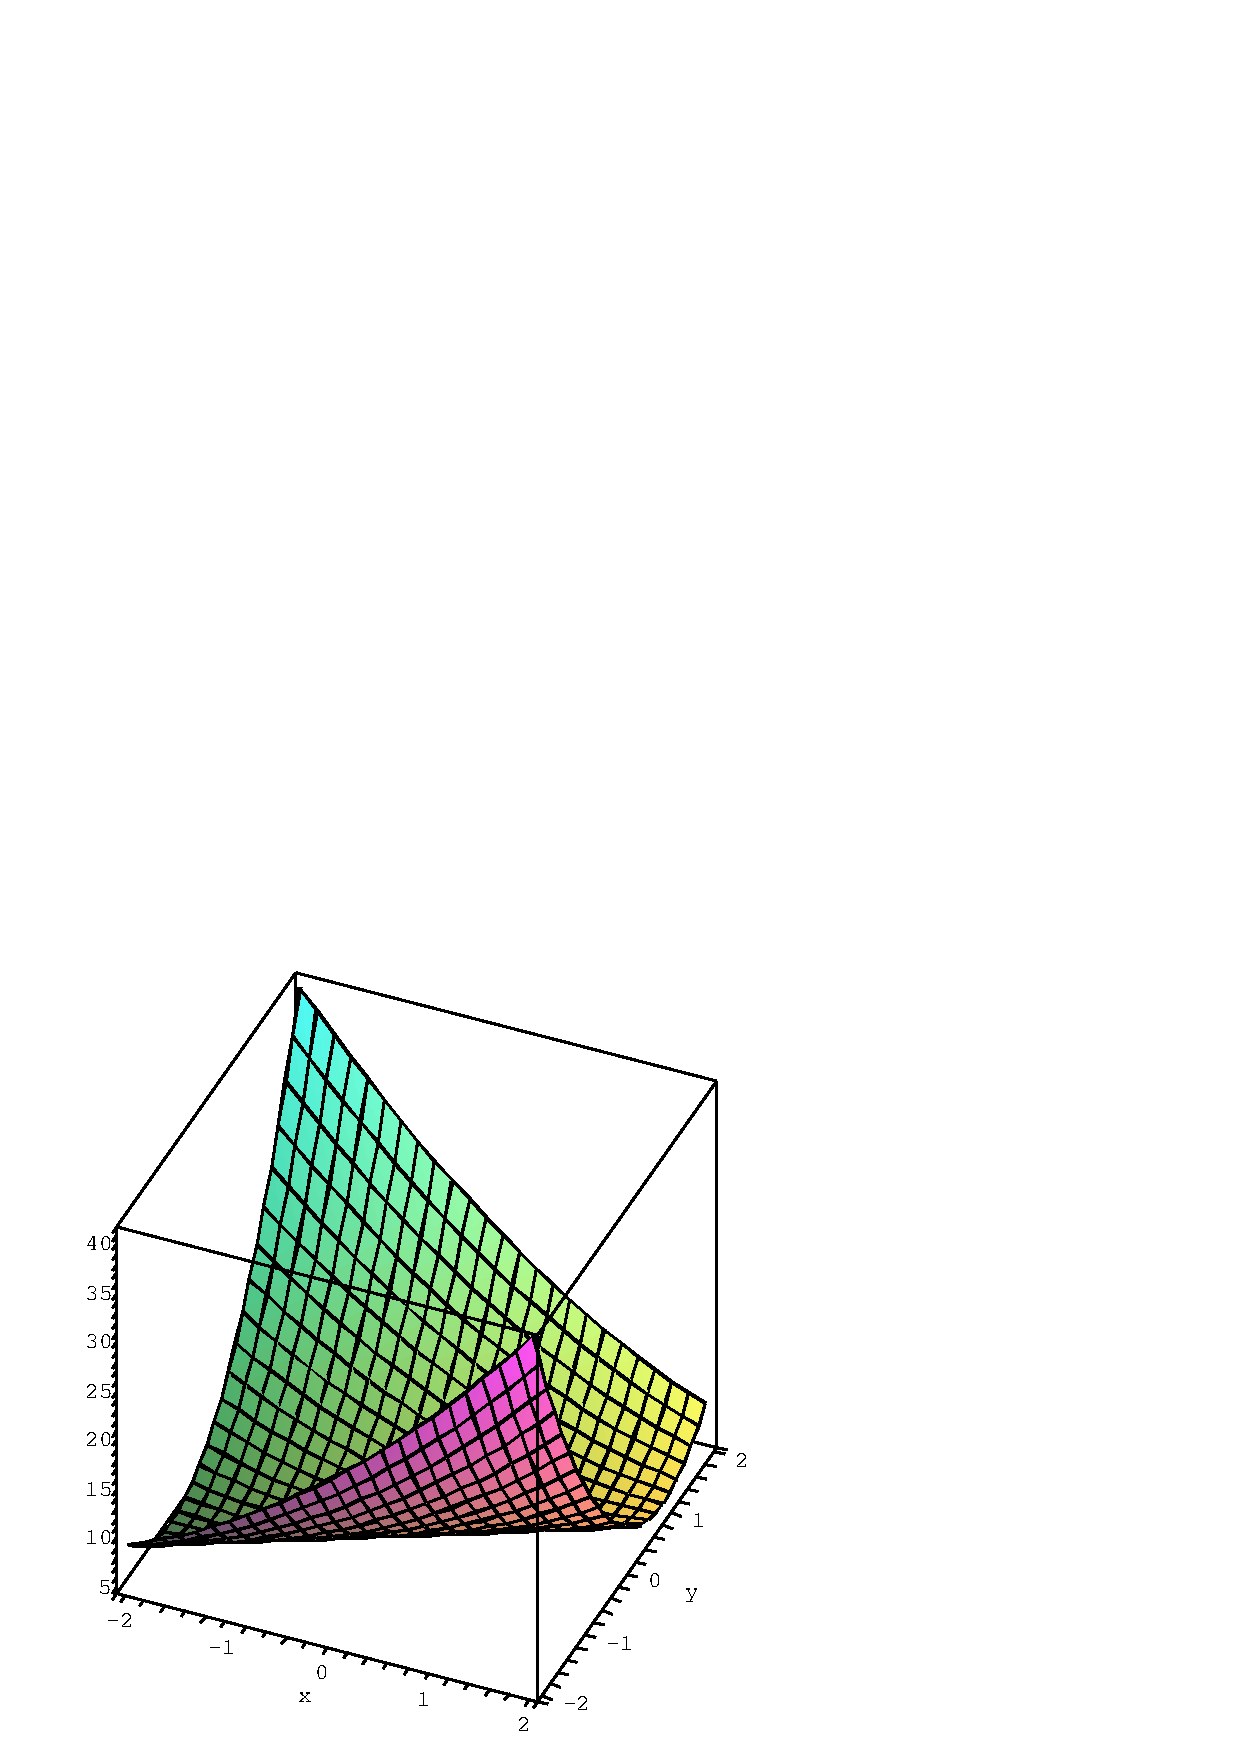
\includegraphics[height=8cm, keepaspectratio]{../images/pdf/zWaf-1.pdf}&
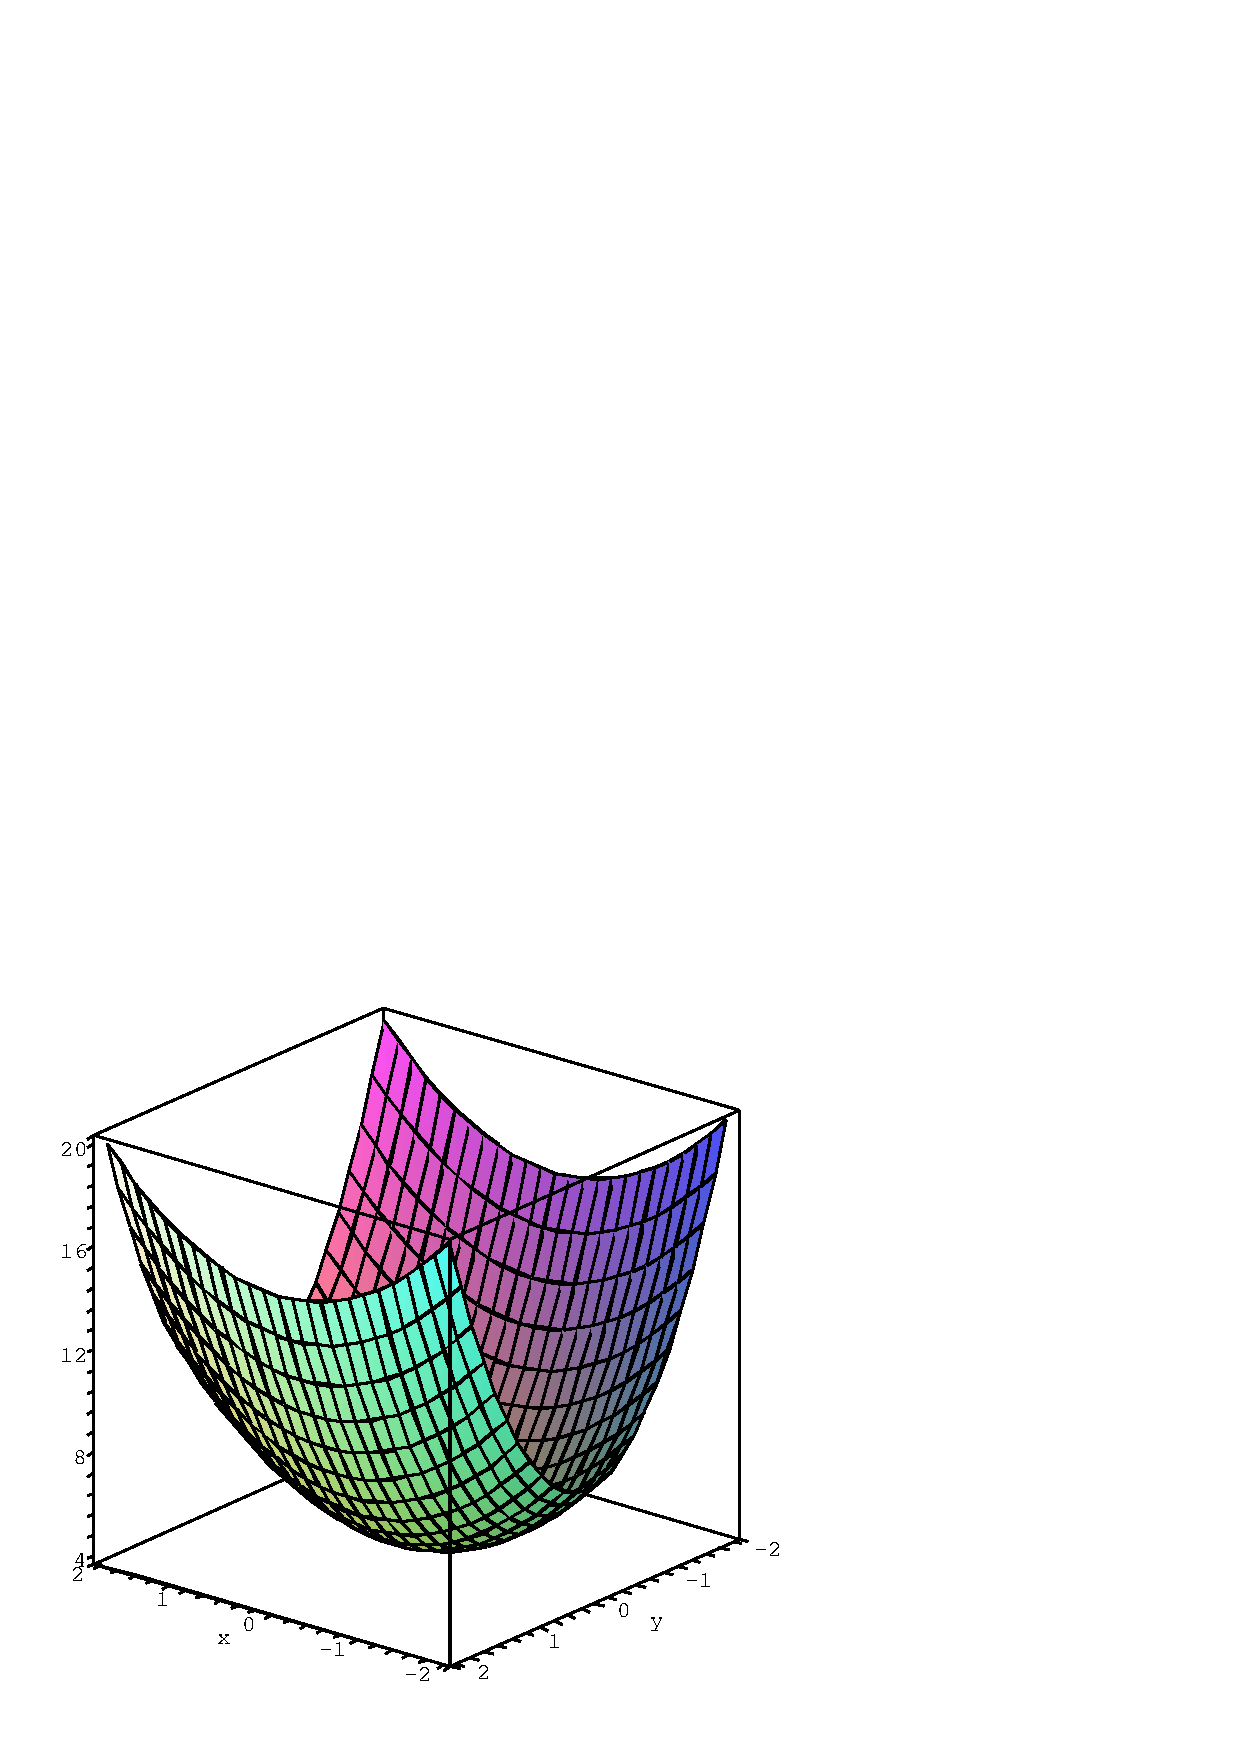
\includegraphics[height=8cm, keepaspectratio]{../images/pdf/zWaf-2.pdf}\\
A&B\\
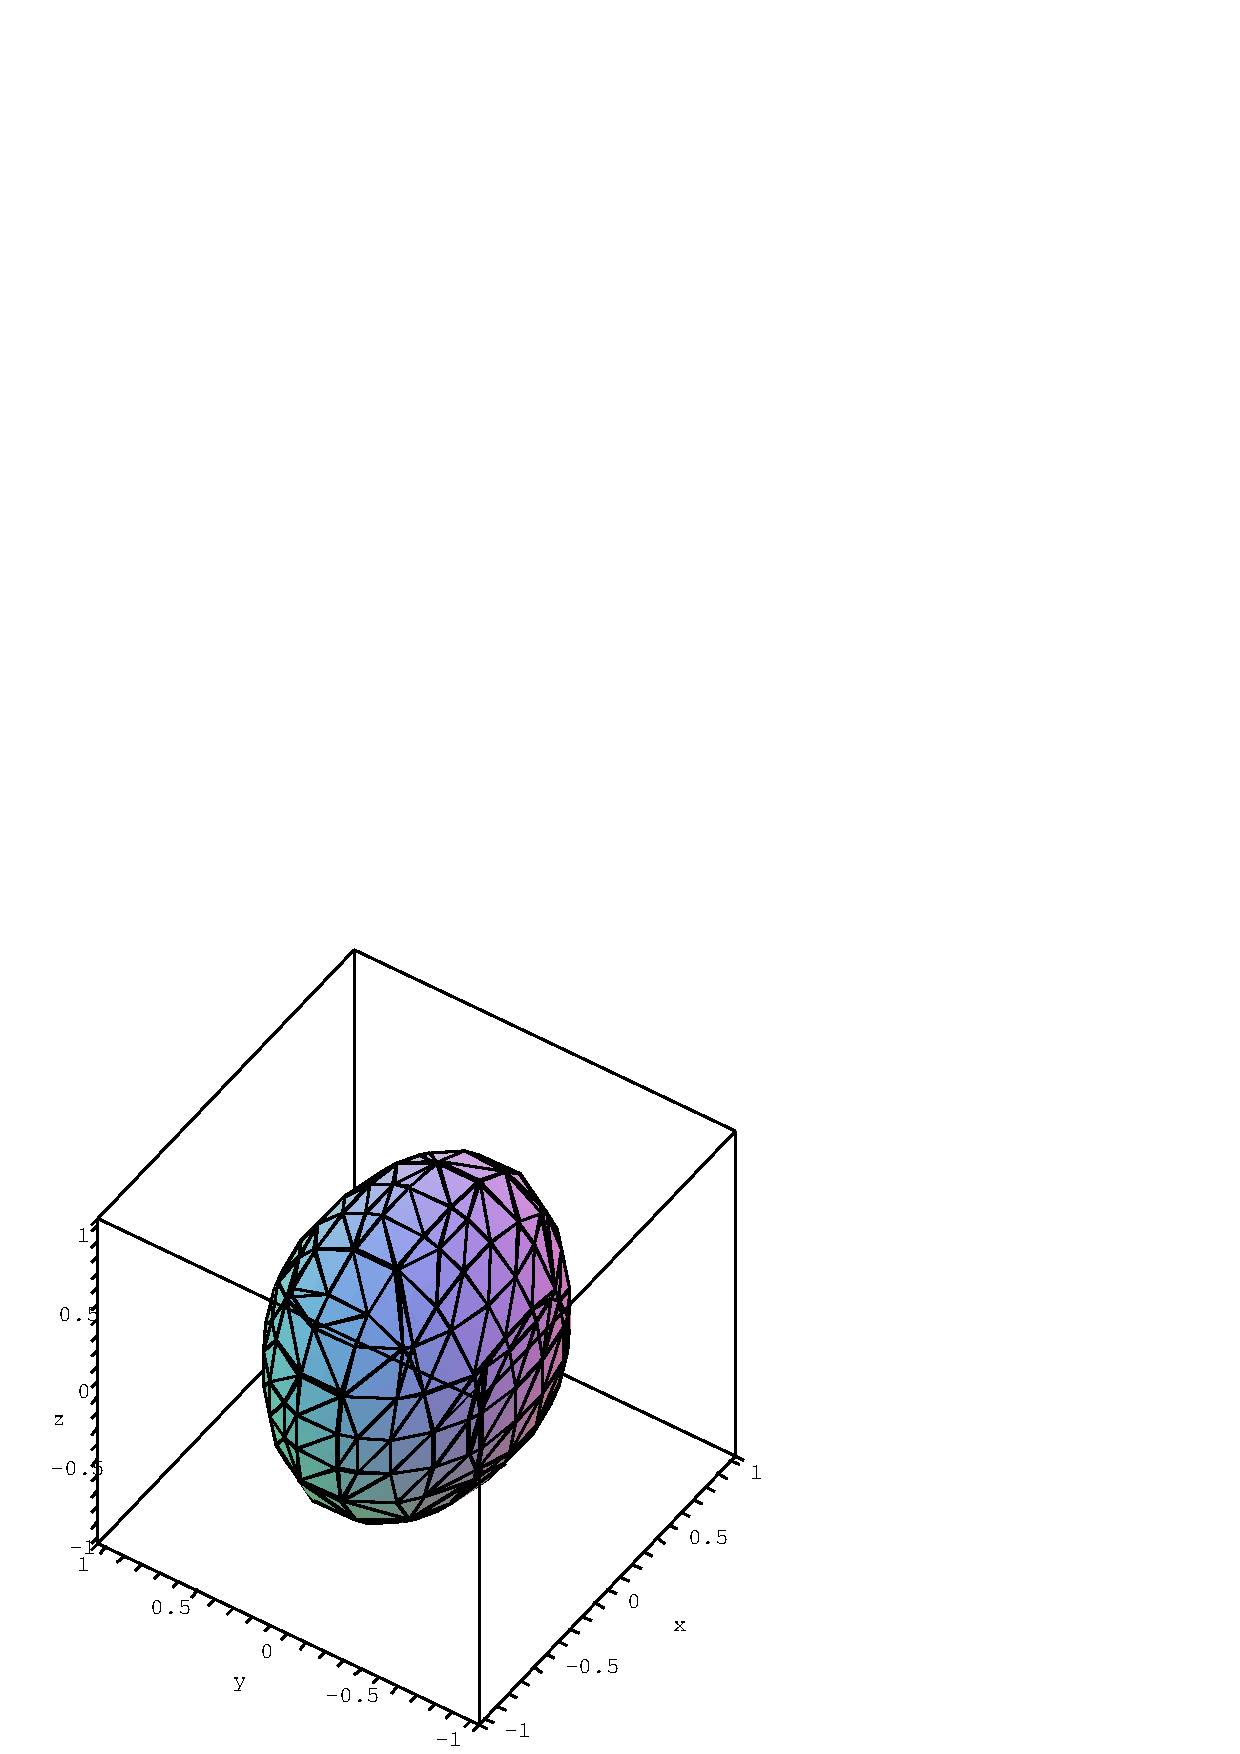
\includegraphics[height=8cm, keepaspectratio]{../images/pdf/zWaf-3.pdf}&
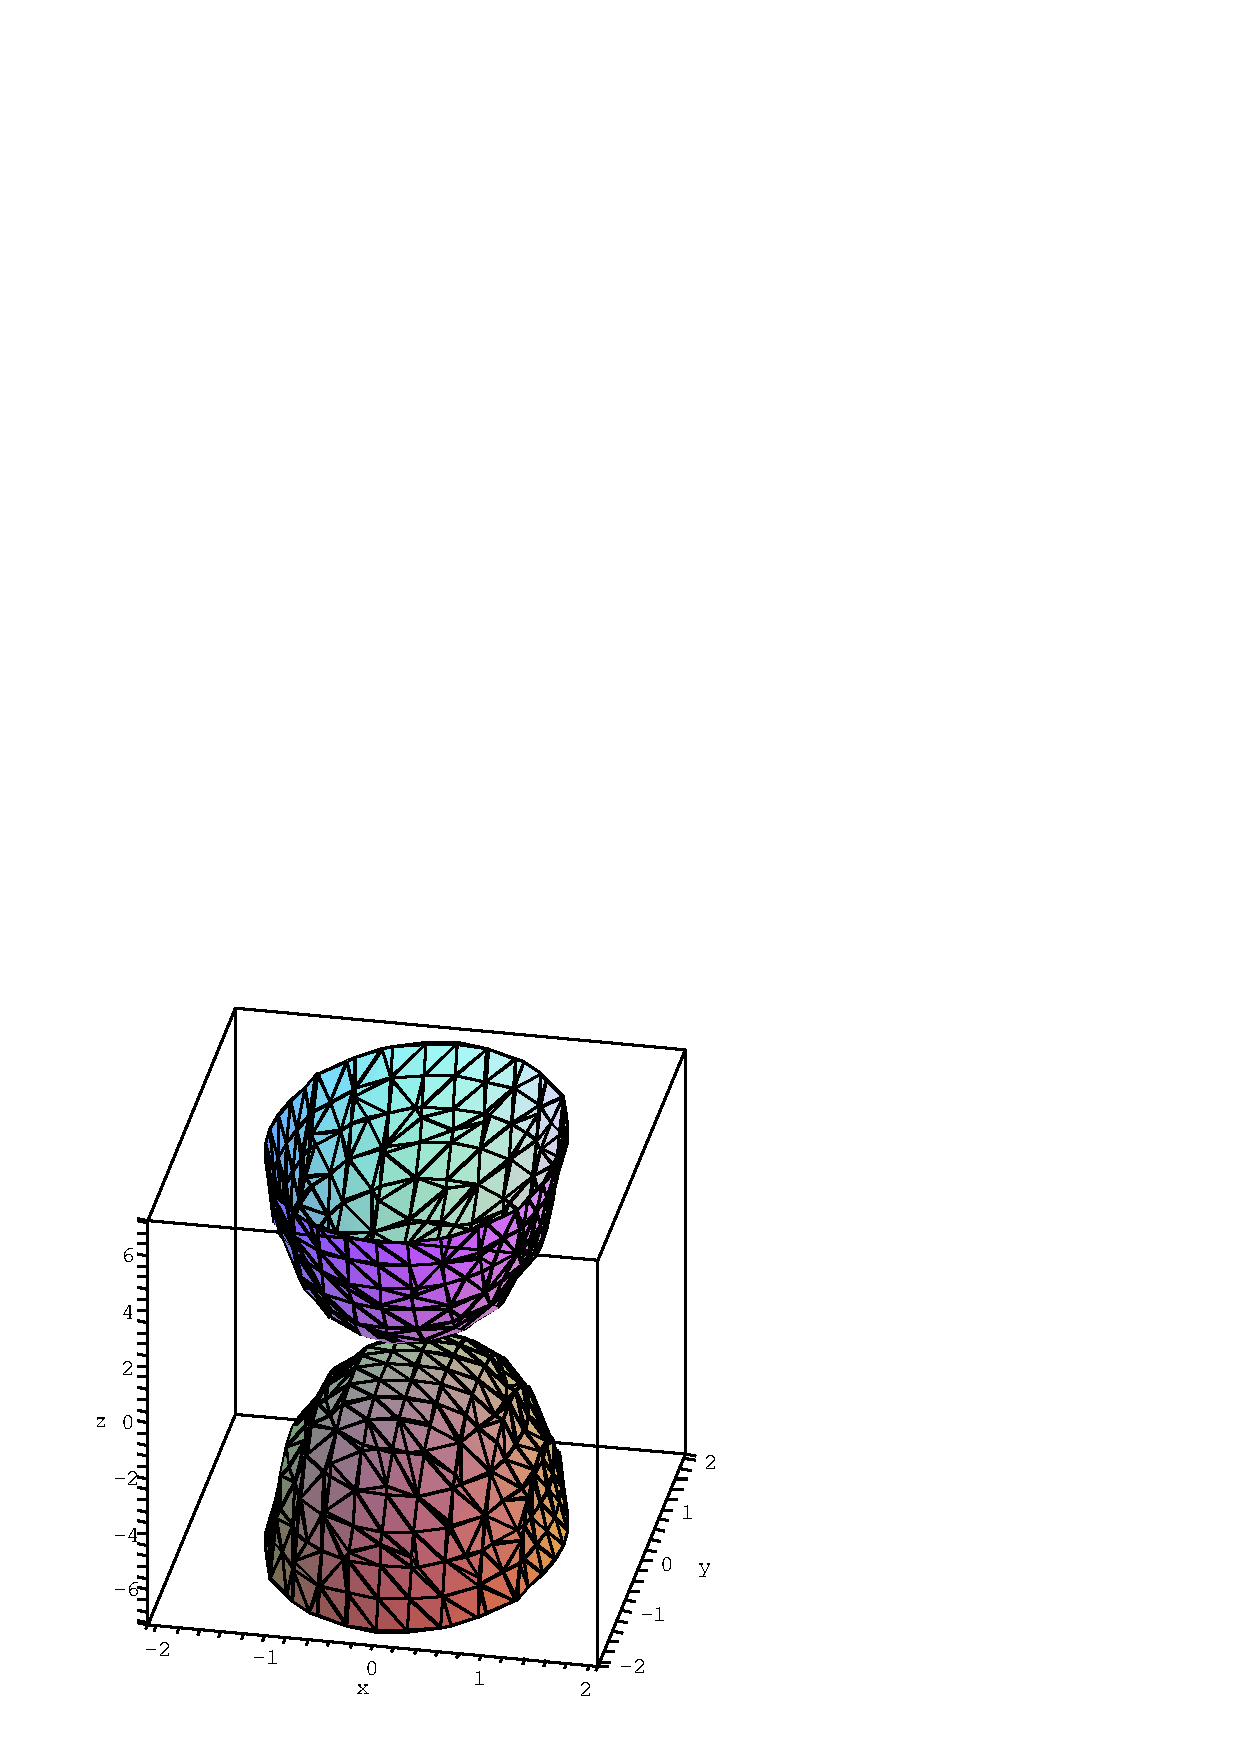
\includegraphics[height=8cm, keepaspectratio]{../images/pdf/zWaf-4.pdf}\\
C&D\end{tabular}
}
}
}
